\documentclass[journal,12pt,twocolumn]{IEEEtran}

\usepackage{enumitem}
\usepackage{amsmath}
\usepackage{amssymb}
\usepackage{gensymb}
\usepackage{graphicx}
\usepackage{txfonts}         
\usepackage{listings}
\usepackage{lstautogobble}
\usepackage{mathtools}
\usepackage{bm}
\usepackage{hyperref}
\usepackage{polynom}
\usepackage{capt-of}
\usepackage{siunitx}
\newcommand{\solution}{\noindent \textbf{Solution: }}
\providecommand{\pr}[1]{\ensuremath{\Pr\left(#1\right)}}
\providecommand{\brak}[1]{\ensuremath{\left(#1\right)}}
\providecommand{\cbrak}[1]{\ensuremath{\left\{#1\right\}}}
\providecommand{\sbrak}[1]{\ensuremath{\left[#1\right]}}
\providecommand{\mean}[1]{E\left[ #1 \right]}
\providecommand{\var}[1]{\mathrm{Var}\left[ #1 \right]}
\providecommand{\der}[1]{\mathrm{d} #1}
\providecommand{\gauss}[2]{\mathcal{N}\ensuremath{\left(#1,#2\right)}}
\providecommand{\mbf}{\mathbf}
\providecommand{\abs}[1]{\left\vert#1\right\vert}
\providecommand{\norm}[1]{\left\lVert#1\right\rVert}
\providecommand{\z}[1]{{\mathcal{Z}}\{#1\}}
\providecommand{\ztrans}{\overset{\mathcal{Z}}{ \rightleftharpoons}}

\providecommand{\parder}[2]{\frac{\partial}{\partial #2} \brak{#1}}

\let\StandardTheFigure\thefigure
\let\vec\mathbf

\numberwithin{equation}{section}
\renewcommand{\thefigure}{\theenumi}
\renewcommand\thesection{\arabic{section}}

\newcommand{\myvec}[1]{\ensuremath{\begin{pmatrix}#1\end{pmatrix}}}
\newcommand{\mydet}[1]{\ensuremath{\begin{vmatrix}#1\end{vmatrix}}}
\newcommand{\define}{\stackrel{\triangle}{=}}

\DeclareMathOperator*{\argmin}{arg\,min}
\DeclareMathOperator*{\argmax}{arg\,max}

\makeatletter
\def\pld@CF@loop#1+{%
    \ifx\relax#1\else
        \begingroup
          \pld@AccuSetX11%
          \def\pld@frac{{}{}}\let\pld@symbols\@empty\let\pld@vars\@empty
          \pld@false
          #1%
          \let\pld@temp\@empty
          \pld@AccuIfOne{}{\pld@AccuGet\pld@temp
                            \edef\pld@temp{\noexpand\pld@R\pld@temp}}%
           \pld@if \pld@Extend\pld@temp{\expandafter\pld@F\pld@frac}\fi
           \expandafter\pld@CF@loop@\pld@symbols\relax\@empty
           \expandafter\pld@CF@loop@\pld@vars\relax\@empty
           \ifx\@empty\pld@temp
               \def\pld@temp{\pld@R11}%
           \fi
          \global\let\@gtempa\pld@temp
        \endgroup
        \ifx\@empty\@gtempa\else
            \pld@ExtendPoly\pld@tempoly\@gtempa
        \fi
        \expandafter\pld@CF@loop
    \fi}
\def\pld@CMAddToTempoly{%
    \pld@AccuGet\pld@temp\edef\pld@temp{\noexpand\pld@R\pld@temp}%
    \pld@CondenseMonomials\pld@false\pld@symbols
    \ifx\pld@symbols\@empty \else
        \pld@ExtendPoly\pld@temp\pld@symbols
    \fi
    \ifx\pld@temp\@empty \else
        \pld@if
            \expandafter\pld@IfSum\expandafter{\pld@temp}%
                {\expandafter\def\expandafter\pld@temp\expandafter
                    {\expandafter\pld@F\expandafter{\pld@temp}{}}}%
                {}%
        \fi
        \pld@ExtendPoly\pld@tempoly\pld@temp
        \pld@Extend\pld@tempoly{\pld@monom}%
    \fi}
\makeatother

\lstset {
	frame=single, 
	breaklines=true,
	columns=fullflexible,
	autogobble=true
}             
   


\begin{document}
                             
\title{ Digital Signal Processing \\ \Large EE3900: Linear Systems and Signal Processing \\ \large Indian Institute of Technology Hyderabad}
\author{Aakash Kamuju \\ \normalsize AI21BTECH11001 \\ \vspace*{20pt} \normalsize 1 Aug 2022}   
 \maketitle 
 \tableofcontents

%\renewcommand{\thefigure}{\thesection.\theenumi}
%\renewcommand{\thetable}{\thesection.\theenumi}

\renewcommand{\thefigure}{\theenumi}
\renewcommand{\thetable}{\theenumi}

%\renewcommand{\theequation}{\thesection}


\bigskip

\begin{abstract}
This manual provides a simple introduction to digital signal processing.
\end{abstract}
\section{Software Installation}
Run the following commands
\begin{lstlisting}
sudo apt-get update
sudo apt-get install libffi-dev libsndfile1 python3-scipy  python3-numpy python3-matplotlib 
sudo pip install cffi pysoundfile 
\end{lstlisting}
\section{Digital Filter}
\begin{enumerate}[label=\thesection.\arabic*
,ref=\thesection.\theenumi]
\item
\label{prob:input}
Download the sound file from  
\begin{lstlisting}
wget https://github.com/kamujuaakash/EE3900/blob/main/codes/Sound_Noise.wav
\end{lstlisting}
%\href{http://tlc.iith.ac.in/img/sound/Sound_Noise.wav}{\url{http://tlc.iith.ac.in/img/sound/Sound_Noise.wav}}  
%in the link given below.
%\linebreak
\item
\label{prob:spectrogram}
You will find a spectrogram at \href{https://academo.org/demos/spectrum-analyzer}{\url{https://academo.org/demos/spectrum-analyzer}}. 
%\end{problem}
%%
%
%%\onecolumn
%%\input{./figs/fir}
%\begin{problem}
Upload the sound file that you downloaded in Problem \ref{prob:input} in the spectrogram  and play.  Observe the spectrogram. What do you find?
\\
%
\solution There are a lot of yellow lines between 440 Hz to 5.1 KHz.  These represent the synthesizer key tones. Also, the key strokes
are audible along with background noise.
% By observing spectrogram, it clearly shows that tonal frequency is under 4kHz. And above 4kHz only noise is present.
\item
\label{prob:output}
Write the python code for removal of out of band noise and execute the code.
\\
\solution
\lstinputlisting{./codes/Cancel_noise.py}
%\begin{figure}[h]
%\centering
%\includegraphics[width=\columnwidth]{enc_block_diag.png}
%\caption{}
%\label{fig:convolution encoder}
%\end{figure}
%\input{block_enc}
\item
The output of the python script in Problem \ref{prob:output} is the audio file Sound\_With\_ReducedNoise.wav. Play the file in the spectrogram in Problem \ref{prob:spectrogram}. What do you observe?
\\
\solution The key strokes as well as background noise is subdued in the audio.  Also,  the signal is blank for frequencies above 5.1 kHz.

\end{enumerate}
\section{Difference Equation}
\begin{enumerate}[label=\thesection.\arabic*,ref=\thesection.\theenumi]
\item Let
\begin{equation}
x(n) = \cbrak{\underset{\uparrow}{1},2,3,4,2,1}
\end{equation}
Sketch $x(n)$.
\\
\solution The following code yields Fig. \ref{fig:3.1}
\begin{lstlisting}
wget https://github.com/kamujuaakash/EE3900/blob/main/codes/3.1.py
\end{lstlisting}
\begin{figure}[!ht]
\begin{center}
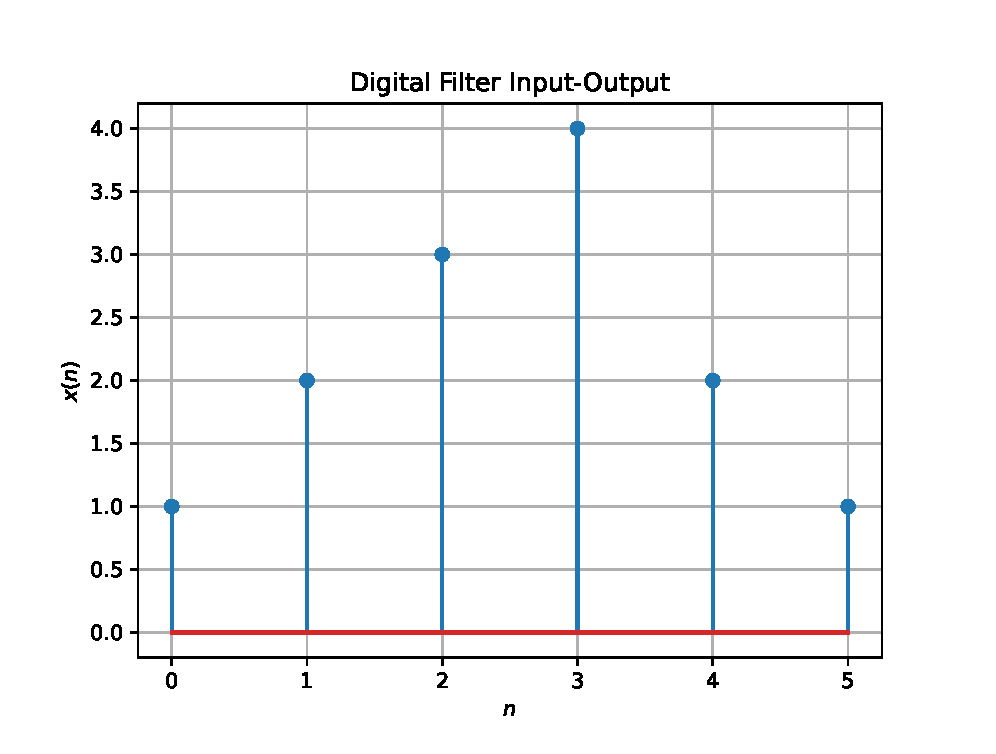
\includegraphics[width=\columnwidth]{./figs/3.1}
\end{center}
\captionof{figure}{}
\label{fig:3.1}	
\end{figure}
\item Let
\begin{multline}
\label{eq:iir_filter}
y(n) + \frac{1}{2}y(n-1) = x(n) + x(n-2), 
\\
 y(n) = 0, n < 0
\end{multline}
Sketch $y(n)$.
\\
\solution The following code yields Fig. \ref{fig:xnyn}.
\begin{lstlisting}
wget https://github.com/kamujuaakash/EE3900/blob/main/codes/xnyn.py
\end{lstlisting}
\begin{figure}[!ht]
\begin{center}
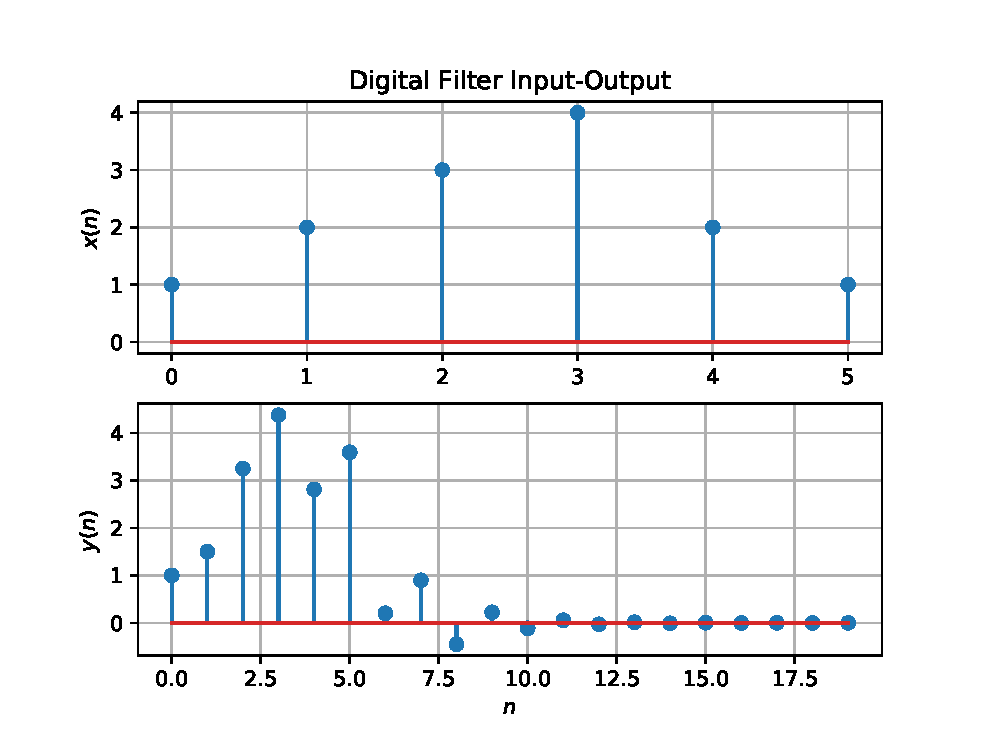
\includegraphics[width=\columnwidth]{./figs/xnyn}
\end{center}
\captionof{figure}{}
\label{fig:xnyn}	
\end{figure}

\end{enumerate}
\section{$Z$-transform}
\begin{enumerate}[label=\thesection.\arabic*]
\item The $Z$-transform of $x(n)$ is defined as
%
\begin{equation}
\label{eq:z_trans}
X(z)={\mathcal {Z}}\{x(n)\}=\sum _{n=-\infty }^{\infty }x(n)z^{-n}
\end{equation}
%
Show that
\begin{equation}
\label{eq:shift1}
{\mathcal {Z}}\{x(n-1)\} = z^{-1}X(z)
\end{equation}
and find
\begin{equation}
	{\mathcal {Z}}\{x(n-k)\} 
\end{equation}
\solution From \eqref{eq:z_trans},
\begin{align}
{\mathcal {Z}}\{x(n-k)\} &=\sum _{n=-\infty }^{\infty }x(n-1)z^{-n}
\\
&=\sum _{n=-\infty }^{\infty }x(n)z^{-n-1} = z^{-1}\sum _{n=-\infty }^{\infty }x(n)z^{-n}
\end{align}
resulting in \eqref{eq:shift1}. Similarly, it can be shown that
%
\begin{equation}
\label{eq:z_trans_shift}
	{\mathcal {Z}}\{x(n-k)\} = z^{-k}X(z)
\end{equation}
\item Obtain $X(z)$ for x(n) define in problem 3.1.
\solution From \eqref{eq:z_trans},
\begin{align}
X(z)&={\mathcal{Z}}\{x(n)\}=\sum_{n=-\infty}^{\infty}x(n)z^{-n}\\
\label{eq:genf}
&=\sum_{n=0}^{\infty}x(n)z^{-n}\\
&=1\cdot z^{-1}+2\cdot z^{-2}+3\cdot z^{-3}+4\cdot z^{-4}+2\cdot z^{-5}+1\cdot z^{-6}\\
&=\frac{z^5+2z^4+3z^3++4z^2+2z+1}{z^6}
\end{align}
\item Find
%
\begin{equation}
H(z) = \frac{Y(z)}{X(z)}
\end{equation}
%
from  \eqref{eq:iir_filter} assuming that the $Z$-transform is a linear operation.
\\
\solution  Applying \eqref{eq:z_trans_shift} in \eqref{eq:iir_filter},
\begin{align}
Y(z) + \frac{1}{2}z^{-1}Y(z) &= X(z)+z^{-2}X(z)
\\
\implies H\brak{z} = \frac{Y(z)}{X(z)} &= \frac{1 + z^{-2}}{1 + \frac{1}{2}z^{-1}}
\label{eq:freq_resp}
\end{align}
%
\item Find the Z transform of 
\begin{equation}
\delta(n)
=
\begin{cases}
1 & n = 0
\\
0 & \text{otherwise}
\end{cases}
\end{equation}
and show that the $Z$-transform of
\begin{equation}
\label{eq:unit_step}
u(n)
=
\begin{cases}
1 & n \ge 0
\\
0 & \text{otherwise}
\end{cases}
\end{equation}
is
\begin{equation}
U(z) = \frac{1}{1-z^{-1}}, \quad \abs{z} > 1
\end{equation}
\solution It is easy to show that
\begin{equation}
\delta(n) \ztrans 1
\end{equation}
and from \eqref{eq:unit_step},
\begin{align}
U(z) &= \sum _{n= 0}^{\infty}z^{-n}
\\
&=\frac{1}{1-z^{-1}}, \quad \abs{z} > 1
\end{align}
using the fomula for the sum of an infinite geometric progression.
%
\item Show that 
\begin{equation}
\label{eq:anun}
a^nu(n) \ztrans \frac{1}{1-az^{-1}} \quad \abs{z} > \abs{a}
\end{equation}
\solution From \eqref{eq:z_trans},
\begin{equation}
{\mathcal {Z}}\{a^nu(n)\} = \sum _{n= -\infty}^{\infty}u(n)\brak{\frac{a}{z}}^{-n}
\end{equation}
From \eqref{eq:unit_step},
\begin{align}
{\mathcal {Z}}\{a^nu(n)\} &= \sum _{n= 0}^{\infty}\brak{\frac{a}{z}}^{-n}\\
&= \frac{1}{1-\frac{a}{z}}\\
&= \frac{1}{1-az^{-1}} \quad \abs{z} > \abs{a}
\end{align}
using the formula for the sum of an infinite geometric progression.

%
\item 
Let
\begin{equation}
H\brak{e^{\j \omega}} = H\brak{z = e^{\j \omega}}.
\end{equation}
Plot $\abs{H\brak{e^{\j \omega}}}$. Is it periodic? If so,find the period. $H(e^{\j \omega})$ is
known as the {\em Discret Time Fourier Transform} (DTFT) of $x(n)$.
\\
\solution 
\begin{align}
H\brak{e^{\j \omega}} &= H\brak{z = e^{\j \omega}}\\
&= \frac{1 + e^{-2 \j \omega}}{1 + \frac{1}{2} e^{-\j \omega}}\\
&= \frac{2\brak{1 + e^{-2 \j \omega}}}{2 + e^{-\j \omega}}\\
&= \frac{2\brak{1 + \cos{2 \omega}-\j \sin{2\omega}}}{2 + \cos{\omega}-\j \sin{ \omega}}\\
&= \frac{2\abs{\brak{2\cos^2 \omega-\j \sin{2\omega}}}}{\abs{2 + \cos{\omega}-\j \sin{ \omega}}}\\
&= \frac{2\sqrt{4\cos^4 \omega+4\sin^2 \omega \cos^2 \omega}}{\sqrt{\brak{2 + \cos \omega}^2+ \sin^2 \omega }}\\
&=\frac{4\cos\omega}{\sqrt{5 + 4\cos \omega}}\\
\abs{H\brak{e^{\j \omega}} }&=\frac{\abs{4\cos\omega}}{\sqrt{5 + 4\cos \omega}}
\end{align}
Since $\abs{H(e^{j\omega})}$ is function of cosine we can say it is periodic.And from the plot \ref{fig:dtft} we can say that it is symmetric about $\omega = 0\brak{\text{even function}}$ and it is periodic with period $2\pi$.You can find the same from the theoritical expression $\abs{H\brak{e^{j \omega}}}$, 
       \begin{align}
         H(e^{\j \omega}) &= H(e^{j(-\omega)})\brak{\text{cos is an even function}}
       \end{align}
    And to find period, the period of $\abs{\cos(\omega)}$ is $\pi$ and the period of $\sqrt{5 + 4\cos\brak{\omega}}$ is $2\pi$. So the period of division of both will be $2\pi$.
     This gives us the period of $\abs{H(e^{j\omega})}$ as $2\pi$
 The following code plots Fig. \ref{fig:dtft}.
\begin{lstlisting}
wget https://github.com/kamujuaakash/EE3900/blob/main/codes/hn.py
\end{lstlisting}
\begin{figure}[!ht]
\centering
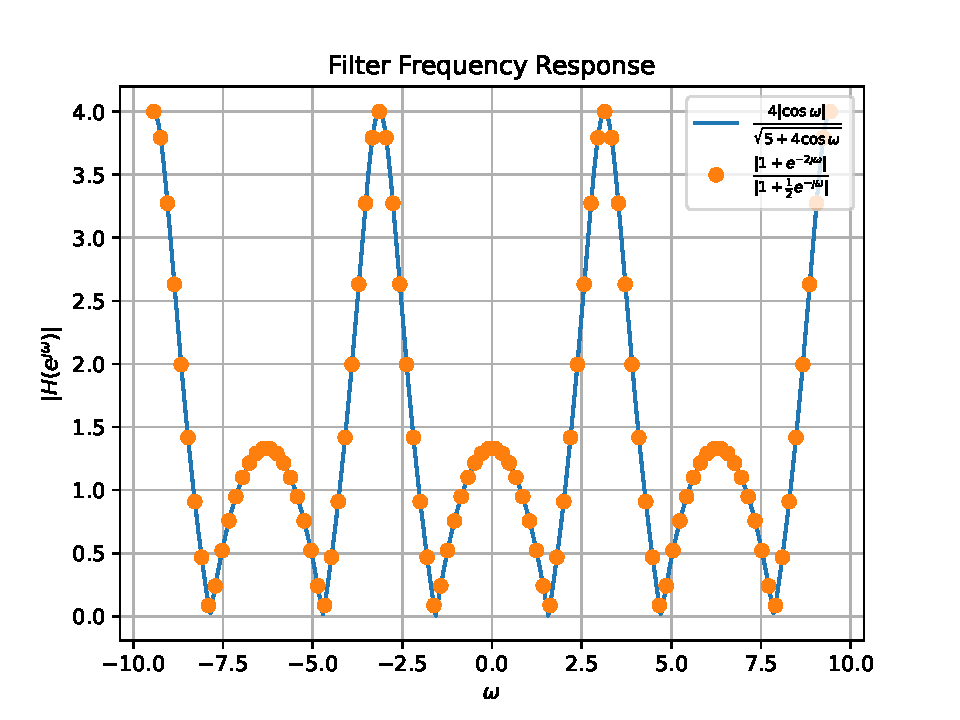
\includegraphics[width=\columnwidth]{./figs/dtft}
\caption{$\abs{H\brak{e^{\j\omega}}}$}
\label{fig:dtft}
\end{figure}


\item Express $h(n)$ in terms of $H\brak{e^{\j\omega}}$	
	
	\solution 
\begin{align}
\int_{-\pi}^{\pi} H(e^{\j\omega}) e^{\j\omega n} d\omega\\
= \int_{-\pi}^{\pi} \sum_{k=-\infty}^\infty h(k)  e^{-\j\omega k} e^{\j\omega n} d\omega\\
= \sum_{k=-\infty}^\infty h(k) \int_{-\pi}^{\pi} e^{\j\omega(n-k)} d\omega
\end{align}	
	Now,
	\begin{align}
		 \int_{-\pi}^{\pi} e^{\j\omega(n-k)} d\omega 
		 &= \begin{cases}
		 	\int_{-\pi}^\pi d\omega & n-k = 0 \\
		 	\left.\frac{\exp\brak{\j\omega(n-k)}}{\j(n-k)}\right|_{-\pi}^\pi & n-k \ne 0
		 \end{cases} \\		 
		 &= \begin{cases}
		 	2\pi & n-k = 0 \\
		 	0 & n-k \ne 0
		 \end{cases} \\
		 &= 2\pi \delta(n-k)
	\end{align}
	
	Thus,
	\begin{align}
		\int_{-\pi}^{\pi} H(e^{\j\omega}) e^{\j\omega n} d \omega &= 2\pi\sum_{k=-\infty}^\infty h(k) \delta(n-k) \\
		&= 2\pi h(n) * \delta(n) \\
		&= 2\pi h(n)
	\end{align}
	
	Therefore, $h(n)$ is given by the inverse DTFT (IDTFT) of $H\brak{e^{\j\omega}}$
	\begin{align}
		h(n) &= \frac{1}{2\pi} \int_{-\pi}^{\pi} H(e^{\j\omega}) e^{\j\omega n}  d \omega 
	\end{align}
\end{enumerate}

\section{Impulse Response}
\begin{enumerate}[label=\thesection.\arabic*]
\item Using long division, 
find
		\begin{align}
			h(n), \quad n < 5
		\end{align}
		for H(z) in 
		\eqref{eq:freq_resp}.\\
\solution 
	\begin{equation}
		H(z) = \frac{1 + z^{-2}}{1 + \frac12 z^{-1}}
	\end{equation}
	Substitute $z^{-1} = x$
	\polylongdiv{1+x^2}{1+\frac12 x}
	
	\begin{align}
		&\implies 1 + z^{-2} = \brak{1 + \frac12 z^{-1}}\brak{-4 + 2z^{-1}} + 5 \\
		&\implies H(z) = -4 + 2z^{-1} + \frac{5}{1 + \frac12 z^{-1}}
	\end{align}
	
	On applying the inverse $Z$-transform on both sides of the equation
	\begin{align}
		H(z) &\ztrans h(n) \\
		-4 &\ztrans -4\delta(n) \\
		2z^{-1} &\ztrans 2\delta(n - 1) \\
		\frac{5}{1 + \frac12 z^{-1}} &\ztrans 5\brak{-\frac12}^n u(n) \\
	\end{align}
	
	Therefore,
	\begin{equation}
		h(n) = -4\delta(n) + 2\delta(n - 1) + 5\brak{-\frac12}^n u(n)
	\end{equation}
\item \label{prob:impulse_resp}
Find an expression for $h(n)$ using $H(z)$, given that 
in \eqref{eq:anun}, given that
\begin{equation}
\label{eq:impulse_resp}
h(n) \ztrans H(z)
\end{equation}
and there is a one to one relationship between $h(n)$ and $H(z)$. $h(n)$ is known as the {\em impulse response} of the
system defined by \eqref{eq:iir_filter}.
\\
\solution From \eqref{eq:freq_resp},
\begin{align}
H(z) &= \frac{1}{1 + \frac{1}{2}z^{-1}} + \frac{ z^{-2}}{1 + \frac{1}{2}z^{-1}}
\\
\implies h(n) &= \brak{-\frac{1}{2}}^{n}u(n) + \brak{-\frac{1}{2}}^{n-2}u(n-2)
\end{align}
using \eqref{eq:anun} and \eqref{eq:z_trans_shift}.

\item Sketch $h(n)$. Is it bounded? Justify theoretically.
\\
\solution 

The following code plots
\begin{figure}[!ht]
\begin{center}
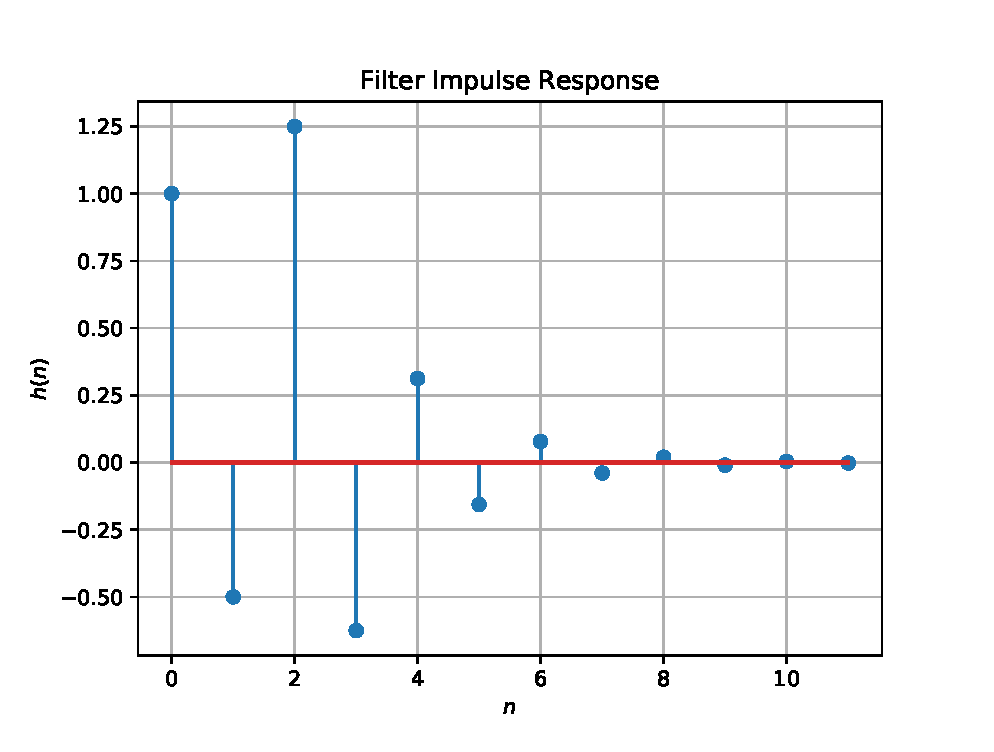
\includegraphics[width=\columnwidth]{./figs/hn}
\end{center}
\captionof{figure}{}
\label{fig:xnyn}	
\end{figure}
\begin{lstlisting}
wget https://github.com/kamujuaakash/EE3900/blob/main/Simulation/codes/5.3.py
\end{lstlisting}

\begin{align}
\lim_{n\to\infty}h(n)&=\lim_{n\to\infty}\brak{-\frac{1}{2}}^{n}u(n) + \lim_{n\to\infty}\brak{-\frac{1}{2}}^{n-2}u(n-2)
\end{align}
\begin{equation}
h(n)
=
\begin{cases}
5\brak{\frac{-1}{2}}^n & n \ge 2
\\
\brak{\frac{-1}{2}}^n & 0\le n < 2
\\
0 & n<0
\end{cases}
\end{equation}
Maximum value and minimum value are always bounded in this case.
$\therefore h(n)$ is bounded

 \item Is it convergent? Justify using the ratio test.
\solution
\begin{align}
h(n+1)&=\brak{-\frac{1}{2}}^{n+1}u(n+1) + \brak{-\frac{1}{2}}^{n-1}u(n-1)
\end{align}
According to ratio test, $L$ is given by $\lim_{n\to \infty}\abs{\frac{h(n+1)}{h(n)}}$, if $L < 1$ then h(n) is convergent.
\begin{align}
L&=\lim_{n\to \infty}\abs{\frac{h(n+1)}{h(n)}}\\
&=\lim_{n\to \infty}\abs{\frac{\brak{-\frac{1}{2}}^{n+1}u(n+1) + \brak{-\frac{1}{2}}^{n-1}u(n-1)}{\brak{-\frac{1}{2}}^{n}u(n) + \brak{-\frac{1}{2}}^{n-2}u(n-2)}}\\
&=\abs{\frac{-\frac{1}{2} + {-\frac{1}{2}}^{-1}}{1 + {-\frac{1}{2}}^-2}}\\
&=\abs{\frac{-\frac{1}{2}-2}{1+4}}\\
&=\abs{\frac{\frac{-5}{2}}{5}}\\
&=\frac{1}{2}
\end{align}
As $L < 1$, $h(n)$ is convergent.

\item The system with $h(n)$ is defined to be stable if
\begin{equation}
\sum_{n=-\infty}^{\infty}h(n) < \infty
\end{equation}
Is the system defined by \eqref{eq:iir_filter} stable for the impulse response in \eqref{eq:impulse_resp}?\\
\solution 
\begin{align}
\sum_{n=-\infty}^{\infty}h(n)&= \sum_{n=0}^{\infty}h(n)\\
&=\sum_{n=0}^{\infty}\brak{-\frac{1}{2}}^{n}u(n) + \sum_{n=0}^{\infty}\brak{-\frac{1}{2}}^{n-2}u(n-2)\\
&=2 \brak{ \frac{1}{1+\frac{1}{2}}}\\
&=\frac{4}{3}
\end{align}
As $\sum_{n=-\infty}^{\infty}h(n)=\frac{4}{3}$ is less than $\infty$, the system defined by (3.2) is stable for the impulse response in (5.1).
%
\item Verify the above result using a python code.
\solution The following code determines if it is convergent or not:
\begin{lstlisting}
wget https://github.com/kamujuaakash/EE3900/blob/main/Simulation/codes/5.5.py
\end{lstlisting}
%
\item 
Compute and sketch $h(n)$ using 
\begin{equation}
\label{eq:iir_filter_h}
h(n) + \frac{1}{2}h(n-1) = \delta(n) + \delta(n-2), 
\end{equation}
%
This is the definition of $h(n)$.
\\
\solution The following code plots Fig. \ref{fig:hndef}. Note that this is the same as Fig. 
\ref{fig:hn}. 
%
\begin{lstlisting}
wget https://github.com/kamujuaakash/EE3900/blob/main/Simulation/codes/5.7.py
\end{lstlisting}
Computing,\\
$h(0)=1$\\
$h(1)=-\frac{1}{2}h(0)$\\
$h(2)=-\frac{1}{2}h(1)+1$\\
Parallely, $h(n)=-\frac{1}{2}h(n-1)$

\begin{figure}[!ht]
\centering
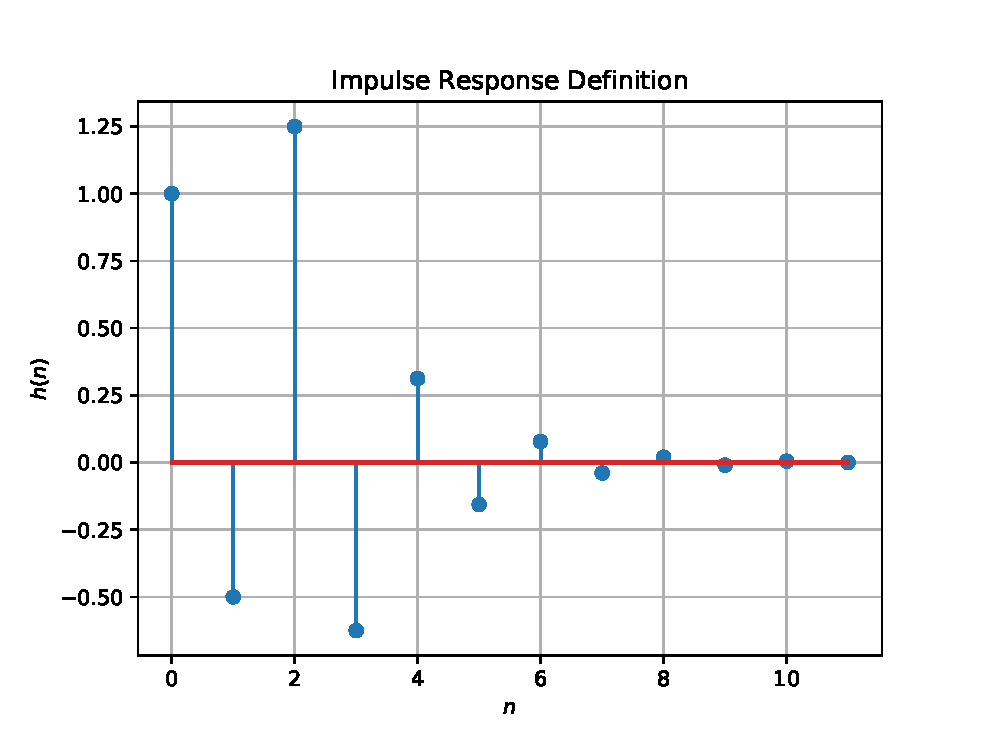
\includegraphics[width=\columnwidth]{./figs/hndef}
\caption{$h(n)$ from the definition}
\label{fig:hndef}
\end{figure}
%
\item Compute 
%
\begin{equation}
\label{eq:convolution}
y(n) = x(n)*h(n) = \sum_{n=-\infty}^{\infty}x(k)h(n-k)
\end{equation}
%
Comment. The operation in \eqref{eq:convolution} is known as
{\em convolution}.
%
\\
\solution The following code plots Fig. \ref{fig:ynconv}. Note that this is the same as 
$y(n)$ in  Fig. 
\ref{fig:xnyn}. 
%
\begin{lstlisting}
wget https://github.com/kamujuaakash/EE3900/blob/main/Simulation/codes/5.8.py
\end{lstlisting}
\begin{figure}[!ht]
\centering
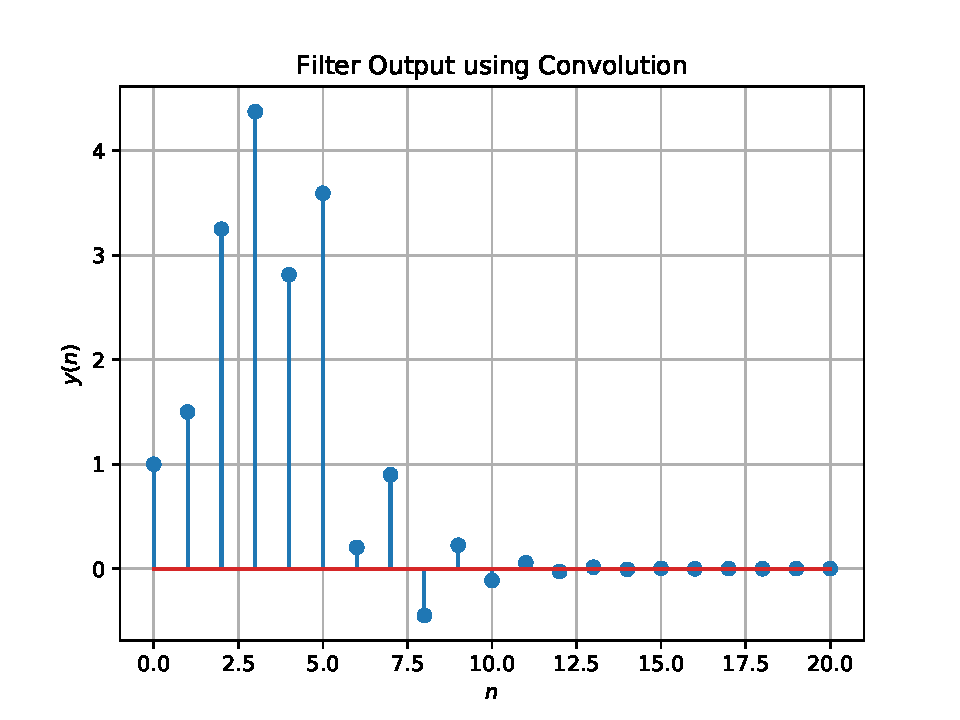
\includegraphics[width=\columnwidth]{./figs/ynconv}
\caption{$y(n)$ from the definition of convolution}
\label{fig:ynconv}
\end{figure}
\item Express the above convolution using a toeplitz matrix.
\solution
\begin{align}
\vec{y} = \vec{x} 
\circledast \vec{h}\\
& \vec{y} = \myvec{ h_1 & 0 & . & . & . & 0 \\ h_2 & h_1 & . & . & . & 0 \\ h_3 & h_2 & h_1 & . & . & 0 \\
 h_{m-1} & . & . & . & h_2 & h_1 \\ 
 h_m & h_{m-1} &. & . & . & h_2 \\ 
 . & . &. & . & . & . \\ 
 . & . & . & . & . & . \\
  0 & 0 & . & . & . & h_m } 
  \myvec{x_1 \\ x_2 \\ . \\ . \\ . \\ . \\ x_n}
\end{align}

\begin{align}
\vec{y}&=\myvec{1 & 0&0 & 0 & 0 & 0 \\ \frac{-1}{2} & 1&0&0&0&0\\\frac{5}{4}&\frac{-1}{2}&1&0&0&0\\\frac{-5}{8}&\frac{5}{4}&\frac{-1}{2}&1&0&0\\\frac{5}{16}&\frac{-5}{8}&\frac{5}{4}&\frac{-1}{2}&1&0\\ \frac{-5}{32}&\frac{5}{16}&\frac{-5}{8}&\frac{5}{4}&\frac{-1}{2}&1\\\frac{5}{64}&\frac{-5}{32}&\frac{5}{16}&\frac{-5}{8}&\frac{5}{4}&\frac{-1}{2}\\ 0&\frac{5}{64}&\frac{-5}{32}&\frac{5}{16}&\frac{-5}{8}&\frac{5}{4}\\0&0&\frac{5}{64}&\frac{-5}{32}&\frac{5}{16}&\frac{-5}{8}\\0&0&0&\frac{5}{64}&\frac{-5}{32}&\frac{5}{16}\\0&0&0&0&\frac{5}{64}&\frac{-5}{32}\\0&0&0&0&0&\frac{5}{64}}\myvec{1\\2\\3\\4\\2\\1}
&=\myvec{1.   \\     1.5\\3.25\\4.375\\2.8125   \\3.59375\\   0.203125\\
  0.9375  \\ -0.390625 \\ 0.3125   \\ 0.     \\	   0.078125}
\end{align}
And this is what we got in \eqref{eq:convolution}
\item Show that
\begin{equation}
y(n) =  \sum_{n=-\infty}^{\infty}x(n-k)h(k)
\end{equation}
\solution Substitute $k\to n-k$ then \begin{align}
y(n) &=  x(n)*h(n)\\
&=\sum_{n=-\infty}^{\infty}x(k)h(n-k)
&= \sum_{n=-\infty}^{\infty}x(n-k)h(k)
\end{align}
\end{enumerate}
%
\section{DFT and FFT}
\begin{enumerate}[label=\thesection.\arabic*]
\item
Compute
\begin{equation}
X(k) \define \sum _{n=0}^{N-1}x(n) e^{-\j2\pi kn/N}, \quad k = 0,1,\dots, N-1
\end{equation}
and $H(k)$ using $h(n)$.
\solution The following code plots Fig. \ref{fig:xkhk}. 
\begin{figure}[!ht]
\centering
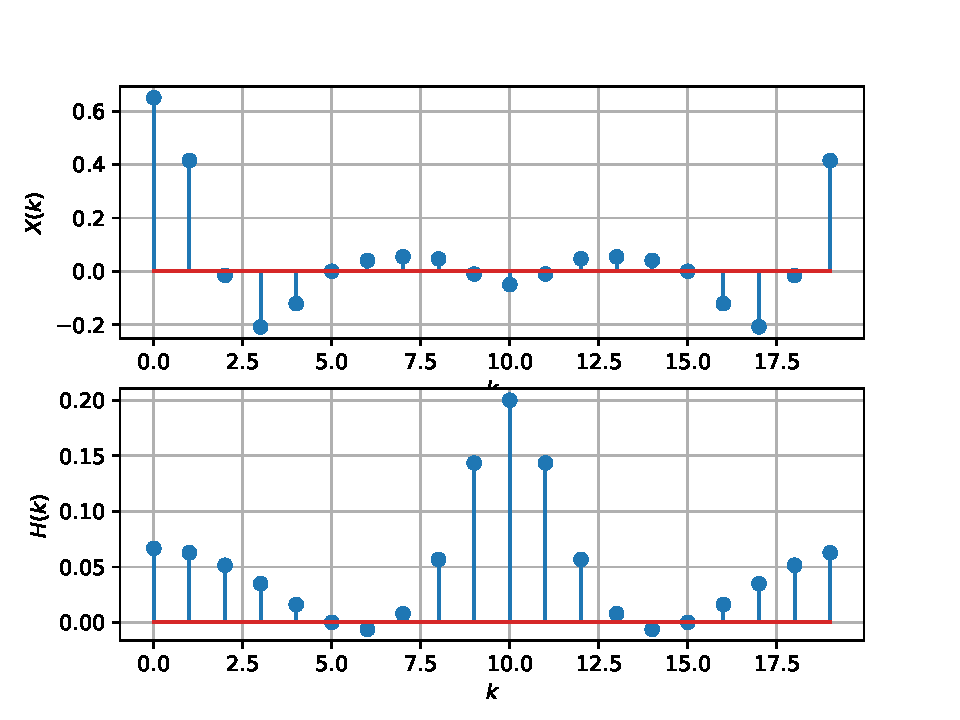
\includegraphics[width=\columnwidth]{./figs/xkhk}
\caption{$X(k) ,H(k)$ from the DFT}
\label{fig:xkhk}
\end{figure}
\begin{lstlisting}
wget https://github.com/kamujuaakash/EE3900/blob/main/codes/xkhkdft.py
\end{lstlisting}
\item Compute 
\begin{equation}
Y(k) = X(k)H(k)
\end{equation}
\solution The following code plots Fig. \ref{fig:yk}. 
\begin{figure}[!ht]
\centering
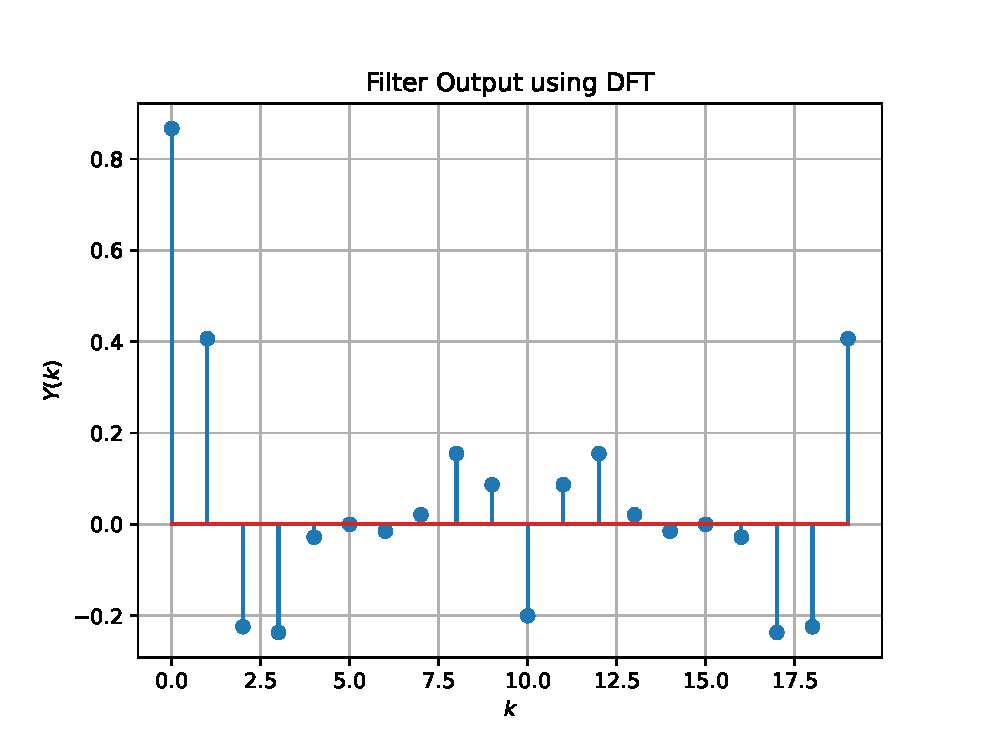
\includegraphics[width=\columnwidth]{./figs/yk}
\caption{$Y(k)$ from the DFT}
\label{fig:yk}
\end{figure}
\begin{lstlisting}
wget https://github.com/kamujuaakash/EE3900/blob/main/codes/ykdft.py
\end{lstlisting}
\item Compute
\begin{equation}
 y\brak{n}={\frac {1}{N}}\sum _{k=0}^{N-1}Y\brak{k}\cdot e^{\j 2\pi kn/N},\quad n = 0,1,\dots, N-1
\end{equation}
\\
\solution The following code plots Fig. \ref{fig:ynconv}. Note that this is the same as 
$y(n)$ in  Fig. 
\ref{fig:xnyn}. 
%
\begin{lstlisting}
wget https://github.com/kamujuaakash/EE3900/blob/main/codes/yndft.py
\end{lstlisting}
\begin{figure}[!ht]
\centering
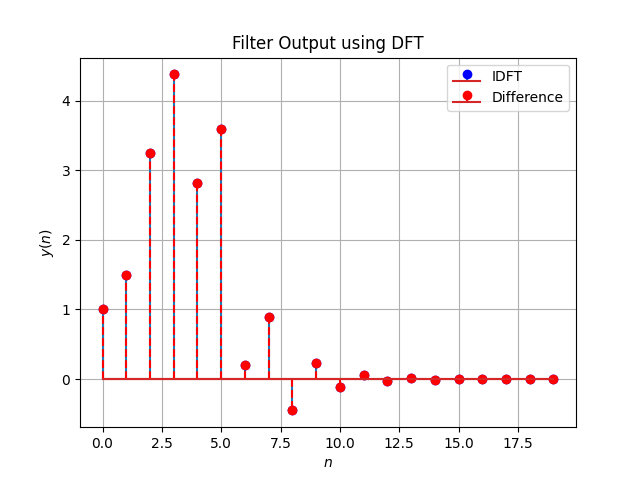
\includegraphics[width=\columnwidth]{./figs/yndft}
\caption{$y(n)$ from the DFT}
\label{fig:yndft}
\end{figure}

\item Repeat the previous exercise by computing $X(k), H(k)$ and $y(n)$ through FFT and 
IFFT.
\solution Download the below python code for the plot $\ref{yn_ifft}$,
  \begin{lstlisting}
wget https://github.com/kamujuaakash/EE3900/blob/main/Simulation/codes/6.4.py
  \end{lstlisting}
  Then run the following command,
   \begin{lstlisting}
python3 6.4.py
   \end{lstlisting}
  \begin{figure}[!ht]
     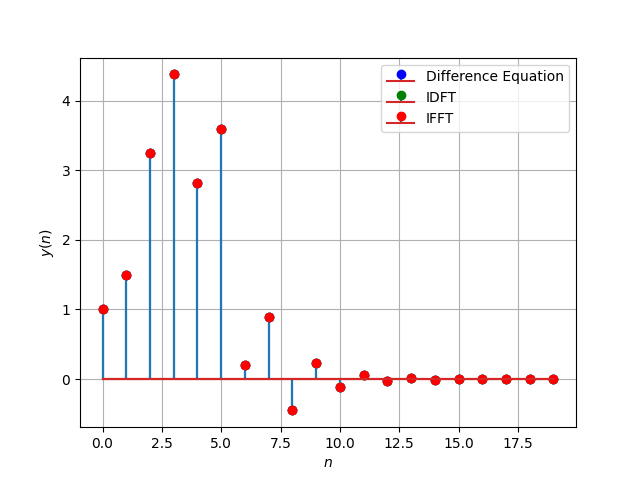
\includegraphics[width=\columnwidth]{./figs/6.4}
     \centering
    \caption{The plot of $y\brak{n}$ using IFFT}
    \label{yn_ifft}
 \end{figure}
%\item Wherever possible, express all the above equations as matrix equations.
\end{enumerate}
%
\section{FFT}
% \subsection{Definitions}
\begin{enumerate}[label=\arabic*.,ref=\thesection.\theenumi]
\numberwithin{equation}{section}
    \item The DFT of $x(n)$ is given by
    \begin{align}
        X(k) \triangleq \sum_{n=0}^{N-1} x(n) e^{-j 2 \pi k n / N}, \quad k=0,1, \ldots, N-1 \label{def:DFT}
    \end{align}
\item Let 
	\begin{align}
W_{N} = e^{-j2\pi/N} \label{eq:twiddle}
	\end{align}
		Then the $N$-point ${ DFT matrix}$ is defined as 
	\begin{align}
		\vec{F}_{N} = \sbrak{W_{N}^{mn}}, \quad 0 \le m,n \le N-1 \label{def:N-point_matrix} 
	\end{align}
	where $W_{N}^{mn}$ are the elements of $\vec{F}_{N}$.
\item Let 
	\begin{align}
		\vec{I}_4 = \myvec{\vec{e}_4^{1} &\vec{e}_4^{2} &\vec{e}_4^{3} &\vec{e}_4^{4} }
	\end{align}
		be the $4\times 4$ identity matrix.  Then the 4 point {\em DFT permutation matrix} is defined as 
	\begin{align}
		\vec{P}_4 = \myvec{\vec{e}_4^{1} &\vec{e}_4^{3} &\vec{e}_4^{2} &\vec{e}_4^{4} } \label{elem_mat}
	\end{align}
\item The 4 point ${ DFT diagonal matrix}$ is defined as 
	\begin{align}
		\vec{D}_4 = diag\myvec{W_{8}^{0} & W_{8}^{1} & W_{8}^{2} & W_{8}^{3}} \label{def-diagonal_matrix}
	\end{align}
\item Show that 
\begin{equation}
    W_{N}^{2}=W_{N/2}
\end{equation}
%    \item Find $\vec{P}_6$.
%    \item Find $\vec{D}_3$.
\solution 
	From $\eqref{eq:twiddle}$,
		\begin{align}
			W_{N} = e^{-j2\pi/N}
		\end{align}
	Consider,
		\begin{align}
			W_{N}^{2} &= \brak{e^{-j2\pi/N}}^2 \\
				  &= e^{-j2\pi/\brak{N/2}} \\
				  &= W_{N/2}\label{result}
		\end{align}
Hence proved.\\
  \item Show that 
\begin{equation}
	\vec{F}_{4}=
\begin{bmatrix}
	\vec{I}_{2} & \vec{D}_{2} \\
\vec{I}_{2} & -\vec{D}_{2}
\end{bmatrix}
\begin{bmatrix}
\vec{F}_{2} & 0 \\
0 & \vec{F}_{2}
\end{bmatrix}
	\vec{P}_{4}
\end{equation}
  \solution From the eq $\eqref{elem_mat}$,
		\begin{align}
                  \vec{P}_4 = \myvec{\vec{e}_4^{1} &\vec{e}_4^{3} &\vec{e}_4^{2} &\vec{e}_4^{4} }
                \end{align}
Clearly $\vec{P}_4$ is an elementary matrix of $\vec{I}_{4}$, so on multiplication with a matrix it will interchange the rows/columns of matrix depending on positions of unit vectors.\\
From that it follows ,
	  \begin{align}
		  \vec{P}_4^2 = \vec{I}_4
	  \end{align}
So it is similar to prove that, 
  \begin{equation} 
	  \vec{F}_{4}\vec{P}_{4}=
\begin{bmatrix}
        \vec{I}_{2} & \vec{D}_{2} \\
\vec{I}_{2} & -\vec{D}_{2}
\end{bmatrix}
\begin{bmatrix}
\vec{F}_{2} & 0 \\
0 & \vec{F}_{2}   
\end{bmatrix}                    
\end{equation}
 Now from $\eqref{def:N-point_matrix}$,
  \begin{align}
	  \vec{F}_{2} &= 
	  \begin{bmatrix}
		  W_2^{0.0} & W_2^{0.1} \\
		  W_2^{1.0} & W_2^{1.1}
	  \end{bmatrix} \\
	  &= \begin{bmatrix}
                  W_2^{0} & W_2^{0} \\
                  W_2^{0} & W_2^{1}
          \end{bmatrix}
  \end{align}
 Using the result $\eqref{result}$, we can write
   \begin{align}
   \vec{F}_{2} &= 
   \begin{bmatrix}
   	W_4^{0} & W_4^{0} \\
   	W_4^{0} & W_4^{2}
   \end{bmatrix} 
\end{align}
 And $\vec{D}_{2}$ is a diagonal matrix,
  \begin{align}
  	\vec{D}_{2} &= diag\brak{W_4^0,W_4^1} \\
  	            &= diag\brak{1,W_4}
  \end{align}
  Then,
   \begin{align}
   	 \vec{D}_2\vec{F}_2 &=\begin{bmatrix}
   	 	                  1 & 0 \\
   	 	                  0 & W_4^{1}
   	                     \end{bmatrix}  
                         \begin{bmatrix}
   	 	                  W_4^{0} & W_4^{0} \\
   	 	                  W_4^{0} & W_4^{2}
   	                      \end{bmatrix} \\
                        &= \begin{bmatrix}
                        	W_4^{0} & W_4^{0} \\
                        	W_4^{1} & W_4^{3}
                          \end{bmatrix}
   \end{align}
And for $k \in \mathcal{N}$ and $N$ be a even integer we know that,
 \begin{align}
 	W_{N}^{Nk} &= 1 \label{result_1}\\
 	W_{N}^{Nk + N/2} &= -1\label{result_2}
 \end{align}
Using that we can write,
  \begin{align}
  	-\vec{D}_2\vec{F}_2 &= \begin{bmatrix}
  		                     W_4^{2} & W_4^{6} \\
  		                     W_4^{3} & W_4^{9}
  	                       \end{bmatrix}
  \end{align}
And from $\eqref{def:N-point_matrix}$,
   \begin{align}
   	\vec{F}_{4} &= \begin{bmatrix}
   		             W_4^0 &  W_4^0& W_4^0 & W_4^0  \\
   		             W_4^0 & W_4^1 & W_4^2 & W_4^3  \\
   		             W_4^0 & W_4^2 & W_4^4 &  W_4^6 \\
   		             W_4^0 & W_4^3 & W_4^6 & W_4^9   
   	               \end{bmatrix}
   \end{align}
And 
   \begin{align}
   	\vec{F}_{4}\vec{P}_{4} &= \begin{bmatrix}
   		                        W_4^0 &  W_4^0& W_4^0 & W_4^0 \\
   		                       W_4^0 & W_4^2 & W_4^1 & W_4^3  \\
   		                       W_4^0 & W_4^4 & W_4^2 &  W_4^6 \\
   		                       W_4^0 & W_4^6 & W_4^3 & W_4^9       
   	                          \end{bmatrix}
   \end{align} 
  This is same as,
        \begin{align}
        	\begin{bmatrix}
        		\vec{F}_{2} & \vec{D}_{2}\vec{F}_{2} \\
        		\vec{F}_{2} & -\vec{D}_{2}\vec{F}_{2}
        	\end{bmatrix}\\
        \implies \begin{bmatrix}
        	\vec{I}_{2} & \vec{D}_{2} \\
        	\vec{I}_{2} & -\vec{D}_{2}
        \end{bmatrix}
        \begin{bmatrix}
        	\vec{F}_{2} & 0 \\
        	0 & \vec{F}_{2}   
        \end{bmatrix}   
        \end{align} 
    Hence proved.
      
\item Show that 
\begin{equation}
\vec{F}_{N}=
\begin{bmatrix}
\vec{I}_{N/2} & \vec{D}_{N/2} \\
\vec{I}_{N/2} & -\vec{D}_{N/2}
\end{bmatrix}
\begin{bmatrix}
\vec{F}_{N/2} & 0 \\
0 & \vec{F}_{N/2}
\end{bmatrix}
\vec{P}_{N}
\end{equation}
\solution As we saw earlier, it is similar to prove that
 \begin{align}
 	\vec{F}_{N}\vec{P}_{N} &= \begin{bmatrix}
 		                      \vec{I}_{N/2} & \vec{D}_{N/2} \\
 		                      \vec{I}_{N/2} & \vec{-D}_{N/2}
 	                          \end{bmatrix}
                              \begin{bmatrix}
                              	\vec{F}_{N/2} &  0 \\
                              	 0             & \vec{F}_{N/2}
                            \end{bmatrix}
 \end{align}
Assuming that $N$ is even, consider LHS
 \begin{align}
 	\vec{F}_{N}\vec{P}_{N} &= \begin{bmatrix}
 		                          W_{N}^{0 \times 0} & W_{N}^{0 \times 2} & ..& W_{N}^{0 \times 1} & W_{N}^{0 \times 3} .. \\
 		                           W_{N}^{1 \times 0} & W_{N}^{1 \times 2 } &..& W_{N}^{1 \times 1} & W_{N}^{1 \times 3} .. \\
 		                          & & ..&&  \\
 		                          & & ..&& \\
 		                          W_{N}^{N/2 \times 0} & W_{N}^{N/2 \times 2 } & ..& W_{N}^{N/2 \times 1} & W_{N}^{N/2 \times 3}..  \\
                                  & & ..&& \\
                                  && ..&&\\
                                  W_{N}^{N-1 \times 0} & W_{N}^{N-1 \times 2 } & .. & W_{N}^{N-1 \times 1} & W_{N}^{N-1 \times 3}..  \\ 
 		                      \end{bmatrix}
 \label{matrix_form}
\end{align}
On multiplying with $\vec{P}_{N} \brak{\text{permutation matrix}}$, the odd-numbered columns of $\vec{F}_{N}$ shifted towards left.\\
 Now we can divide the above matrix $\eqref{matrix_form}$, into four sub-matrices as,
   \begin{align}
   	           & = \begin{bmatrix}
                       \sbrak{W_{N}^{n\times 2m}} & \sbrak{W_{N}^{n\times\brak{2m + 1}}} \\ \\
                       \sbrak{W_{N}^{(n + \frac{N}{2}) \times (2m) }} & \sbrak{W_{N}^{(n + \frac{N}{2}) \times (2m + 1)}}
                    \end{bmatrix}\\
               & \text{where}, 0 \leq n,m \leq \frac{N}{2} - 1 \nonumber \\
               & = \begin{bmatrix}
               	        \sbrak{\brak{W_{N}^{n\times m}}^2} & \sbrak{W_{N}^{n}\brak{W_{N}^{n\times m}}^2} \\ \\
               			\sbrak{W_{N}^{Nm}\brak{W_{N}^{n \times m}}^2} & \sbrak{W_{N}^{Nm + N/2}W_{N}^{n}\brak{W_{N}^{n \times m}}^2}
               	   \end{bmatrix}
   \end{align}
Using $\eqref{result_1}$, $\eqref{result_2}$ and $\eqref{result}$
 \begin{align}
 	  & =  \begin{bmatrix}
 	  	       \sbrak{W_{\frac{N}{2}}^{n\times m}} & \sbrak{W_{N}^{n}W_{\frac{N}{2}}^{n\times m}}\\ \\
 	  	       \sbrak{W_{\frac{N}{2}}^{n\times m}} & \sbrak{-W_{N}^{n}W_{\frac{N}{2}}^{n\times m}}
 	       \end{bmatrix}
 \end{align}
Now from def $\eqref{def:N-point_matrix}$ and $\eqref{def-diagonal_matrix}$, we can write,
  \begin{align}
  	   & =  \begin{bmatrix}
  	  	      \vec{F}_{\frac{N}{2}} &\vec{D}_{\frac{N}{2}}\vec{F}_{\frac{N}{2}}\\
  	  	       \vec{F}_{\frac{N}{2}}& -\vec{D}_{\frac{N}{2}}\vec{F}_{\frac{N}{2}}
  	        \end{bmatrix} \\
    \implies 	\vec{F}_{N}\vec{P}_{N} &= \begin{bmatrix}
                                          	\vec{I}_{N/2} & \vec{D}_{N/2} \\
    	                                    \vec{I}_{N/2} & \vec{-D}_{N/2}
                                          \end{bmatrix}
                                         \begin{bmatrix}
    	                                  \vec{F}_{N/2} &  0 \\
                                              	0       & \vec{F}_{N/2}
                                         \end{bmatrix}
  \end{align}  
Hence proved.\\
\textbf{Note :} If we want to do the above matrix decomposition recursively the value of $N$ should in the form of $2^{k}$.
          \item Find 
    \begin{align}
	     \vec{P}_4 \vec{x}
    \end{align}
\solution Let $\vec{x}$,
       \begin{align}
       	\vec{x} &= \begin{bmatrix}
       		        x(0) \\ 
       	         	x(1) \\ 
       		        x(2) \\ 
       		        x(3)
       	           \end{bmatrix}
       \end{align}
     and $\vec{P}_4$ is 4 - point permutation matrix.\\
    So,
    \begin{align}
    	\vec{P}_{4}\vec{x} &= \begin{bmatrix}
                               1 & 0 & 0 & 0 \\
                               0 & 0 & 1 & 0 \\
                               0 & 1 & 0 & 0 \\
                               0 & 0 & 0 & 1   		
     	                      \end{bmatrix}
                              \begin{bmatrix}
                              	x(0) \\ 
                              	x(1) \\ 
                              	x(2) \\ 
                              	x(3)
                              \end{bmatrix} \\
                          &= \begin{bmatrix}
                          	   x(0) \\
                          	   x(2) \\
                          	   x(1) \\
                          	   x(3)
                             \end{bmatrix} 
    \end{align}
\item Show that 
    \begin{align}
	    \vec{X} = \vec{F}_N \vec{x}
	    \label{eq:dft-mat-def}
    \end{align}
		where $\vec{x}, \vec{X}$ are the vector representations of $x(n), X(k)$ respectively.\\
\solution From $\eqref{def:DFT}$,
   \begin{align}
   	X(k) &= \sum_{n=0}^{N-1} x(n) W^{kn}
   \end{align}
  Now we will try to convert the above expression into matrix equations,
   \begin{align}
   	&X(0) = \sum_{n=0}^{N-1} x(n) W^{0.n} \\
   	     &= \myvec{W^{0.0}\\ W^{0.1} \\ W^{0.2} \\ W^{0.(N-1)}}^T\myvec{
   	     	                                                x(0)\\
   	     	                                                x(1)\\
   	     	                                                x(2)\\
   	     	                                                 .\\
   	     	                                                 .\\
   	     	                                                x(N-1)
   	     	                                               }
    \end{align}
    \begin{align}
   &X(1) = \myvec{W^{1.0} \\ W^{1.1} \\ W^{1.2} \\ W^{1.(N-1)}}^T\myvec{
                                                         	x(0)\\
   	                                                        x(1)\\
   	                                                        x(2)\\
   	                                                         .\\
   	                                                         .\\
   	                                                       x(N-1)
                                                           }\\
         &.\nonumber \\
         &. \nonumber 
     \end{align}
     \begin{align}
   &X(N-1) = \myvec{W^{(N-1)\times0} \\W^{(N-1)\times1}\\ W^{(N-1)\times2}\\  W^{(N-1)\times(N-1)}}^T\myvec{
                                  x(0)\\
   	                              x(1)\\
   	                              x(2)\\
   	                               .\\
   	                               .\\
   	                             x(N-1)
                                }\\
  &\vec{X} = \nonumber\\ &\begin{bmatrix}
  		W_N^{0\times0}&W_N^{0\times1}&..&W_N^{0\times N-1}\\
  		..&..&..&..\\
  		W_N^{N-1 \times 0}&W_N^{N-1 \times 1}&..&W_N^{N-1 \times N-1}
  	\end{bmatrix}\myvec{
  	x(0)\\
  	x(1)\\
  	x(2)\\
  	.\\
  	.\\
  	x(N-1)
  }
  \end{align}
From def $\eqref{def:N-point_matrix}$,
 \begin{align}
 	\vec{X} &= \vec{F}_{N}\vec{x}
 \end{align}
 Hence proved.
\item Derive the following Step-by-step visualisation  of
8-point FFTs into 4-point FFTs and so on
\begin{equation}
\begin{bmatrix}
X(0) \\ 
X(1) \\ 
X(2) \\ 
X(3)
\end{bmatrix}
=
\begin{bmatrix}
X_{1}(0) \\ 
X_{1}(1)\\ 
X_{1}(2)\\
X_{1}(3)\\
\end{bmatrix}
+
\begin{bmatrix}
W^{0}_{8} & 0 & 0 & 0\\
0 & W^{1}_{8} & 0 & 0\\
0 & 0 & W^{2}_{8} & 0\\
0 & 0 & 0 & W^{3}_{8}
\end{bmatrix}
\begin{bmatrix}
X_{2}(0) \\ 
X_{2}(1) \\ 
X_{2}(2) \\
X_{2}(3)
\end{bmatrix}
\label{8to4_1}
\end{equation}
\begin{equation}
\begin{bmatrix}
X(4) \\ 
X(5) \\ 
X(6) \\ 
X(7)
\end{bmatrix}
=
\begin{bmatrix}
X_{1}(0) \\ 
X_{1}(1)\\ 
X_{1}(2)\\
X_{1}(3)\\
\end{bmatrix}
-
\begin{bmatrix}
W^{0}_{8} & 0 & 0 & 0\\
0 & W^{1}_{8} & 0 & 0\\
0 & 0 & W^{2}_{8} & 0\\
0 & 0 & 0 & W^{3}_{8}
\end{bmatrix}
\begin{bmatrix}
X_{2}(0) \\ 
X_{2}(1) \\ 
X_{2}(2) \\
X_{2}(3)
\end{bmatrix}
\label{8to4_2}
\end{equation}
4-point FFTs into 2-point FFTs
\begin{equation}
\begin{bmatrix}
X_{1}(0) \\ 
X_{1}(1)\\ 
\end{bmatrix}
=
\begin{bmatrix}
X_{3}(0) \\ 
X_{3}(1)\\ 
\end{bmatrix}
+
\begin{bmatrix}
W^{0}_{4} & 0\\
0 & W^{1}_{4}
\end{bmatrix}
\begin{bmatrix}
X_{4}(0) \\ 
X_{4}(1) \\ 
\end{bmatrix}
\end{equation}
\label{4to2_1}
\begin{equation}
\begin{bmatrix}
X_{1}(2) \\ 
X_{1}(3)\\ 
\end{bmatrix}
=
\begin{bmatrix}
X_{3}(0) \\ 
X_{3}(1)\\ 
\end{bmatrix}
-
\begin{bmatrix}
W^{0}_{4} & 0\\
0 & W^{1}_{4}
\end{bmatrix}
\begin{bmatrix}
X_{4}(0) \\ 
X_{4}(1) \\ 
\end{bmatrix}
\label{4to2_2}
\end{equation}
\begin{equation}
\begin{bmatrix}
X_{2}(0) \\ 
X_{2}(1)\\ 
\end{bmatrix}
=
\begin{bmatrix}
X_{5}(0) \\ 
X_{5}(1)\\ 
\end{bmatrix}
+
\begin{bmatrix}
W^{0}_{4} & 0\\
0 & W^{1}_{4}
\end{bmatrix}
\begin{bmatrix}
X_{6}(0) \\ 
X_{6}(1) \\ 
\end{bmatrix}
\label{4to2_3}
\end{equation}
\begin{equation}
\begin{bmatrix}
X_{2}(2) \\ 
X_{2}(3)\\ 
\end{bmatrix}
=
\begin{bmatrix}
X_{5}(0) \\ 
X_{5}(1)\\ 
\end{bmatrix}
-
\begin{bmatrix}
W^{0}_{4} & 0\\
0 & W^{1}_{4}
\end{bmatrix}
\begin{bmatrix}
X_{6}(0) \\ 
X_{6}(1) \\ 
\end{bmatrix}
\label{4to2_4}
\end{equation}
\begin{equation}
P_{8}
\begin{bmatrix}
x(0) \\ 
x(1) \\ 
x(2) \\ 
x(3) \\ 
x(4) \\ 
x(5) \\
x(6) \\
x(7)
\end{bmatrix}
 = 
\begin{bmatrix}
x(0) \\ 
x(2) \\ 
x(4) \\ 
x(6) \\
x(1) \\ 
x(3) \\ 
x(5) \\
x(7)
\end{bmatrix}\label{P_8}
\end{equation}
\begin{equation}
P_{4}
\begin{bmatrix}
x(0) \\ 
x(2) \\ 
x(4) \\ 
x(6) \\
\end{bmatrix}
 = 
\begin{bmatrix}
x(0) \\ 
x(4) \\ 
x(2) \\
x(6)
\end{bmatrix}\label{P4_1}
\end{equation}
\begin{equation}
P_{4}
\begin{bmatrix}
x(1) \\ 
x(3) \\ 
x(5) \\
x(7)
\end{bmatrix}
 = 
\begin{bmatrix}
x(1) \\ 
x(5) \\ 
x(3) \\ 
x(7) \\
\end{bmatrix}\label{P4_2}
\end{equation}
Therefore,
\begin{equation}
\begin{bmatrix}
X_{3}(0) \\ 
X_{3}(1)\\ 
\end{bmatrix}
= F_{2}
\begin{bmatrix}
x(0) \\ 
x(4) \\ 
\end{bmatrix}
\end{equation}
\begin{equation}
\begin{bmatrix}
X_{4}(0) \\ 
X_{4}(1)\\ 
\end{bmatrix}
= F_{2}
\begin{bmatrix}
x(2) \\ 
x(6) \\ 
\end{bmatrix}
\end{equation}
\begin{equation}
\begin{bmatrix}
X_{5}(0) \\ 
X_{5}(1)\\ 
\end{bmatrix}
= F_{2}
\begin{bmatrix}
x(1) \\ 
x(5) \\ 
\end{bmatrix}
\end{equation}
\begin{equation}
\begin{bmatrix}
X_{6}(0) \\ 
X_{6}(1)\\ 
\end{bmatrix}
= F_{2}
\begin{bmatrix}
x(3) \\ 
x(7) \\ 
\end{bmatrix}
\end{equation}
\solution The 8-point FFT can be expressed as,
 \begin{align}
 	X(k) &= \sum_{0}^{7}x(n)e^{\frac{-2\pi kn}{8}} \\
 	     &= \sum_{0}^{3}x(2n)e^{\frac{-2 \pi kn}{4}} + \sum_{1}^{3}e^{\frac{-2 \pi k\brak{2n+1}}{8}} \\
 	     &= \sum_{0}^{3}x(2n)e^{\frac{-2 \pi kn}{4}} + e^{\frac{-2 \pi k}{8}}\sum_{1}^{3}x(2n)e^{\frac{-2 \pi kn}{4}}
  \end{align}
 Call these 4 - point FFTs as $X_1$ and $X_2$,
  \begin{align}
  	X(k) & =X_1(k) + W_{8}^kX_2(k)
  \end{align}  
Now consider,
  \begin{align}
  	X(k+4) &= X_1(k+4)  + W_{8}^{k + 4}X_2(k+4)\\
           & = X_1(k) -W_{8}^kX_2(k) \label{8to4} 	      
   \end{align}
Since the twiddle factors along with $X_1$ and $X_2$ are of 4-point $X_1(k+4) =X_1(k)$ and $X_2(k+4) = X_2(k)$. \\
With that $\eqref{8to4}$ we can see how $\eqref{8to4_1}$ and $\eqref{8to4_2}$ are derived.\\
Now consider these 4-point FFTs,
 \begin{align}
 	X_1(k) &= \sum_{0}^{1}x(4n)e^{\frac{-j 2\pi nk}{2}} + e^{\frac{-j2\pi k}{4}}\sum_{0}^{1}x(4n+2)e^{\frac{-j2\pi nk}{2}} \\
 		   &= X_3(k) + W_4^kX_4(k)
 	\end{align}
 where, $X_3(k)$ and $X_4(k)$ are 2-point FFTs of $x_1(n) = x_1(4n)$ and $x_2(n) = x(4n+2)$.\\
 And you can see that,
  \begin{align}
  	X_1(k+2) &= X_3(k) - W_{4}^kX_4(k)
  \end{align}
With that we can see how we got $\eqref{4to2_1}$ and $\eqref{4to2_2}$. \\
And similarly we can write the 2-point FFTs from $X_2(k)$ as $X_5(k)$  and $X_6(k)$ of subsequences $x(4n+1)$ and $x(4n+3)$.\\
With that we can get $\eqref{4to2_3}$ and $\eqref{4to2_4}$. \\
Mathematically we can write these 2-point FFTs as,
\begin{equation}
	\begin{bmatrix}
		X_{3}(0) \\ 
		X_{3}(1)\\ 
	\end{bmatrix}
	= F_{2}
	\begin{bmatrix}
		x(0) \\ 
		x(4) \\ 
	\end{bmatrix}
\end{equation}
\begin{equation}
	\begin{bmatrix}
		X_{4}(0) \\ 
		X_{4}(1)\\ 
	\end{bmatrix}
	= F_{2}
	\begin{bmatrix}
		x(2) \\ 
		x(6) \\ 
	\end{bmatrix}
\end{equation}
\begin{equation}
	\begin{bmatrix}
		X_{5}(0) \\ 
		X_{5}(1)\\ 
	\end{bmatrix}
	= F_{2}
	\begin{bmatrix}
		x(1) \\ 
		x(5) \\ 
	\end{bmatrix}
\end{equation}
\begin{equation}
	\begin{bmatrix}
		X_{6}(0) \\ 
		X_{6}(1)\\ 
	\end{bmatrix}
	= F_{2}
	\begin{bmatrix}
		x(3) \\ 
		x(7) \\ 
	\end{bmatrix}
	\end{equation}
where, the subsequences required for each 2-point FFT can be obtained from $\eqref{P_8}$ , $\eqref{P4_1}$ and $\eqref{P4_2}$.
\item For 
    \begin{align}
	    \vec{x} = \myvec{1\\2\\3\\4\\2\\1}
        \label{eq:equation1}
    \end{align}
    compute the DFT  
		using 
	    $\eqref{eq:dft-mat-def}$\\
\solution Download the below python code,
 \begin{lstlisting}
 wget https://github.com/Charanyash/EE3900-Digital_Signal_Processing/blob/master/Sound%201/Codes/X_k_dft.py
 \end{lstlisting} 
Then run the following command on terminal,
\begin{lstlisting}
python3 X_k_dft.py
\end{lstlisting}
The plot of DFT can be seen in Fig \ref{DFT_matrix}
\begin{figure}[!h]
	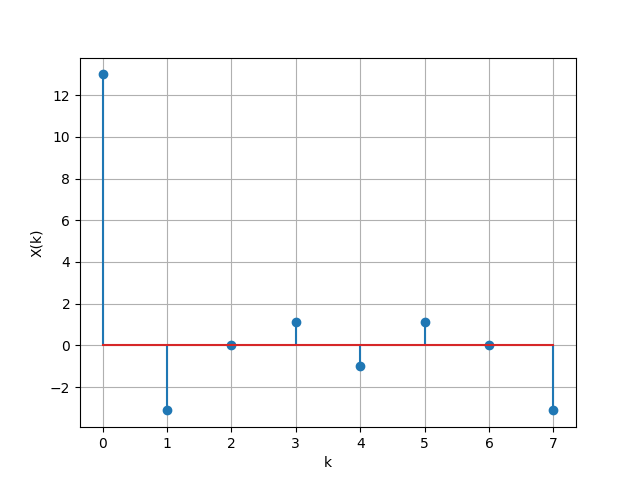
\includegraphics[width = \columnwidth]{figs/X_k_dft.png}
	\centering
	\caption{DFT using DFT matrix}
	\label{DFT_matrix}
\end{figure}
    \item Repeat the above exercise using the FFT
	    after zero padding $\vec{x}$.\\
	\solution Download the below python code,
	\begin{lstlisting}
wget https://github.com/Charanyash/EE3900-Digital_Signal_Processing/blob/master/Sound%201/Codes/X_k_fft.py
	\end{lstlisting} 
	Then run the following command on terminal,
	\begin{lstlisting}
python3 X_k_fft.py
	\end{lstlisting}
	The plot of DFT can be seen in Fig \ref{DFT_fft}
	\begin{figure}[!ht]
		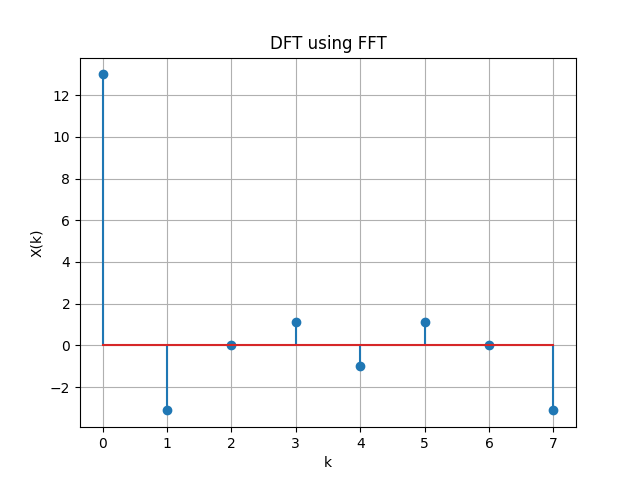
\includegraphics[width = \columnwidth]{figs/X_k_fft.png}
		\centering
		\caption{FFT using Matrix decompostion}
		\label{DFT_fft}
	\end{figure}
%	    \eqref{eq:fft-mat-def}
\item Write a C program to compute the 8-point FFT. \\
 \solution Download the C code from the following link 
  \begin{lstlisting}
wget https://github.com/Charanyash/EE3900-Digital_Signal_Processing/blob/master/Sound%201/Codes/X_k_fft.c 
  \end{lstlisting}
Then run the following command,
\begin{lstlisting}
cc X_k_fft.c -lm
./a.out
\end{lstlisting}
Download the below python code which uses fft.dat file from the C code.
\begin{lstlisting}
wget https://github.com/Charanyash/EE3900-Digital_Signal_Processing/blob/master/Sound%201/Codes/X_k_8point.py
\end{lstlisting}
Then run the following command for the plot,
\begin{lstlisting}
python3 X_k_8point.py
\end{lstlisting}
You will get output of DFT of $x(n)$.
\begin{figure}[!ht]
	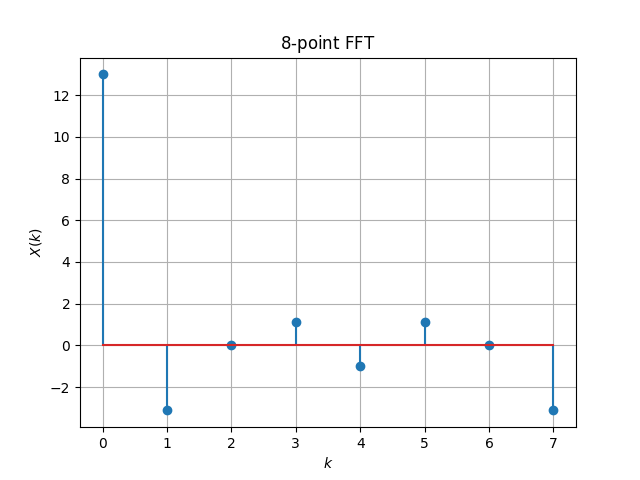
\includegraphics[width = \columnwidth]{figs/X_k_8point.png}
	\centering
	\caption{FFT using C code}
	\label{DFT_fft}
\end{figure}
 \end{enumerate}
\section{Exercises}
Answer the following questions by looking at the python code in Problem \ref{prob:output}.
\begin{enumerate}[label=\thesection.\arabic*]
\item
The command
\begin{lstlisting}
output_signal = signal.lfilter(b, a, input_signal)
	\end{lstlisting}
in Problem \ref{prob:output} is executed through the following difference equation
\begin{equation}
\label{eq:iir_filter_gen}
 \sum _{m=0}^{M}a\brak{m}y\brak{n-m}=\sum _{k=0}^{N}b\brak{k}x\brak{n-k}
\end{equation}
%
where the input signal is $x(n)$ and the output signal is $y(n)$ with initial values all 0. Replace
\textbf{signal.filtfilt} with your own routine and verify.
%
\item Repeat all the exercises in the previous sections for the above $a$ and $b$.
\item What is the sampling frequency of the input signal?
\\
\solution
Sampling frequency(fs)=44.1kHZ.
\item
What is type, order and  cutoff-frequency of the above butterworth filter
\\
\solution
The given butterworth filter is low pass with order=2 and cutoff-frequency=4kHz.
%
\item
Modifying the code with different input parameters and to get the best possible output.
%
\end{enumerate}
\end{document}